\documentclass[12pt,letterpaper]{article}
\usepackage{amsmath,amsthm,amsfonts,amssymb,amscd}
\usepackage{fullpage}
\usepackage{graphicx}
\usepackage{lastpage}
\usepackage{enumerate}
\usepackage{fancyhdr}
\usepackage{hyperref}
\usepackage{mathrsfs}
\usepackage{xcolor}
\usepackage[margin=3cm]{geometry}
\setlength{\parindent}{0.0in}
\setlength{\parskip}{0.05in}

% Edit these as appropriate
\newcommand\course{STA561/CS571}
\newcommand\semester{Fall 2013}     % <-- current semester
\newcommand\hwnum{1}                  % <-- homework number
\newcommand\yourname{Matt Dickenson} % <-- your name
\newcommand\login{mcd31}           % <-- your NetID
\newcommand\hwdate{Due: 11 September, 2013}           % <-- HW due date

\newenvironment{answer}[1]{
  \subsubsection*{Problem #1}
}


\pagestyle{fancyplain}
\headheight 35pt
\lhead{\yourname\ \texttt{\login}\\\course\ --- \semester}
\chead{\textbf{\Large Homework \hwnum}}
\rhead{\hwdate}
\headsep 10pt

\begin{document}

\noindent \emph{Homework Notes:} I worked with Josh Cutler on this homework. To look up density functions I used \url{http://en.wikipedia.org/wiki/Poisson_distribution} and \url{http://en.wikipedia.org/wiki/Uniform_distribution_(continuous)}. 

\begin{answer}{1}
For two dice $X_1$ and $X_2$, the probability of getting a 5 is $P(X_i=5)=\frac{1}{6}$. We can get the probability of getting a 5 on either die by $P(X_1=5 \cup X_2=5)=\frac{1}{6}+\frac{1}{6}-\frac{1}{36}=\mathbf{\frac{11}{36}}$ (where the subtraction term eliminates the double-counted portion). 
\end{answer}

\begin{answer}{2} 

Let $d$ denote the disease state, $nd$ denote ``not disease'', $+$ a positive test result, and $-$ a negative test result.

\begin{eqnarray}
\pi_1(d | +) &=& {{p(+|d) \pi_0(d)} \over p(+)} \\
&=& {{p(+ | d) \pi_0(d) } \over { p(+ |d) \pi_0(d) + p(+ | nd)}} \\
&=& {{0.9 \times 0.001} \over {0.9 \times 0.001 + 0.2 \times 0.999}} \\
&=& 0.00448
\end{eqnarray}
\end{answer}

\begin{answer}{3}
\paragraph{a)} For the probability desnity function, $x$ has a density of ${1 \over {\frac{1}{2}-0}}=2$ if $x \in \lbrack 0, \frac{1}{2} \rbrack$ and $0$ otherwise. 
\paragraph{b)} The density of the pdf at $x=0.00027$ given $a=0, b=\frac{1}{2}$ is 2.
\paragraph{c)} $\int_{0.00027}^{0.00027} 2 dx=2-2=0$. For a continuous distribution the probability at any point has probability $\approx 0$. 
\end{answer}

\newpage
\begin{answer}{4}
\paragraph{a)} Exponential family distributions can be written in the form:
\[
p(x|\lambda) = h(x) \exp(\eta^T T(x) - A(\eta)) 
\]
If we take the Poisson parameterization as 
\[
{\lambda^x \over x!} \times e^{-\lambda}
\]
then we can write out its exponential form using
\begin{eqnarray}
\eta &=& \log \lambda \\
h(x) &=& {1 \over x!} \\
T(x) &=& x \\
A(\eta) &=& e^{\eta} = \lambda
\end{eqnarray}
as
\begin{eqnarray}
p(x|\lambda) &=& {1 \over x!} \exp((\log \lambda)x - \exp{\eta}) \\
&=& {1 \over x!} \exp((\log \lambda)x - \lambda) \\
&=& {1 \over x!} \lambda^x \exp(- \lambda)
\end{eqnarray}
which is equivalent to our original parameterization. 

\paragraph{b)} As shown above, $T(x)=x$.

\paragraph{c)} As shown above, $A(\eta)=e^{\eta}=\lambda$.

\paragraph{d)} For our response function (to translate from $\eta$ to $\lambda$), we use $\lambda=e^\eta$ (the inverse of $\eta = \log \lambda$). 

\paragraph{e)} To get $E[X]$ we can differentiate the log partition function $A(\eta)=e^{\eta}$:
\begin{eqnarray}
E[X] &=& {\partial \over \partial \eta} e^{\eta} \\
&=& e^{\eta} \\
&=& \lambda
\end{eqnarray}

For $Var(X)$ we take the second derivative:
\begin{eqnarray}
Var(X) &=& {\partial^2 \over \partial \eta^2} e^{\eta} \\
&=& {\partial \over \partial \eta} e^{\eta} \\
&=& e^{\eta} \\ 
&=& \lambda
\end{eqnarray}

\paragraph{f)}
We can obtain the MLE estimate of $\lambda$, $\hat{\lambda}$, by taking the first derivative of the exponential familiy parameterization and setting it to zero:
\begin{eqnarray}
0 &=& {\partial \over \partial \eta} ( \log h(x) + \eta \sum_{i=1}^N T(X_i) - n e^{\eta}) \\
&=& 0 + \sum_{i=1}^N T(X_i) - n e^{\eta} \\
&=& \sum_{i=1}^N x_i - n \lambda \\
n\hat{\lambda} &=& \sum_{i=1}^N x_i \\
\hat{\lambda} &=& \frac{1}{n} \sum_{i=1}^N x_i \\
&=& \bar{x}
\end{eqnarray}

\paragraph{g)} For $\lambda \sim Ga(\alpha_0, \beta_0)$ and $X \sim Pois(\lambda)$, the posterior hyperparameters on $\lambda$ are $\alpha_1 = \alpha_0 + \sum_{i=1}^n x_i, \beta_1 = \beta_0 +n$ (thanks to the conjugacy of the Gamma and Poisson distributions). We can find the MAP of $\lambda$ using the mode of this gamma posterior: $\alpha_0 + \sum_{i=1}^n x_i - 1 \over \beta_0 +n$. As a sanity check, it can be seen that with small prior hyperparamters, as we get more data the MAP estimate converges to the MLE estimate in part (f). 

\end{answer}


\begin{answer}{5}

\paragraph{a)} The histogram of data with 25 bins is shown below:

\begin{center}
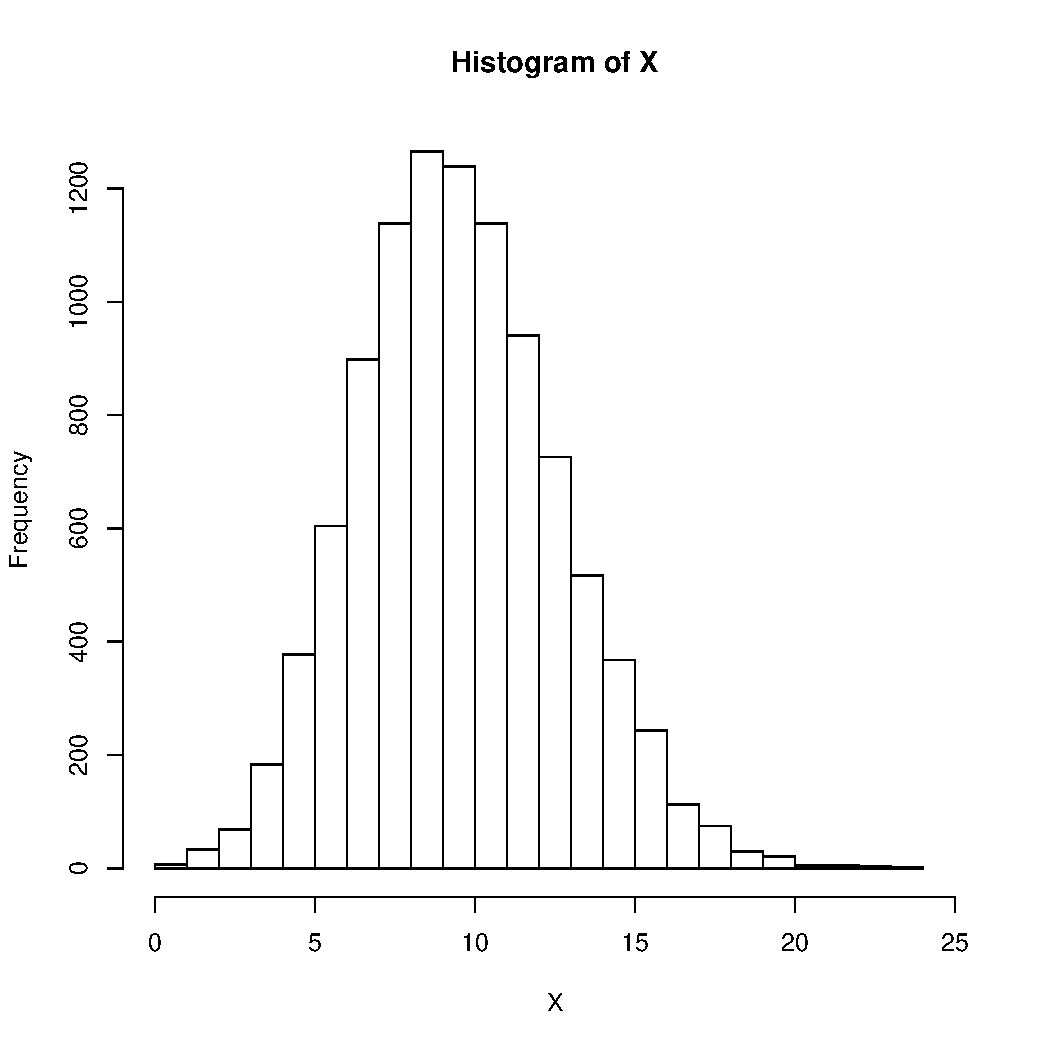
\includegraphics[scale=0.5]{hist5a.pdf}
\end{center}

\paragraph{b)} $\hat{\lambda}=10.0171$

\paragraph{c)} $\alpha=1, \beta=1,$ MAP($\lambda$) = $10.0161$

\paragraph{d)} $\alpha=100, \beta=1,$ MAP($\lambda$) = $10.026$

\paragraph{e)} $\alpha=10, \beta=1,$ MAP($\lambda$) = $10.017$

\paragraph{f)} Given the relatively large amount of data we have (relative to the magnitude of the hyperparameters), the $\alpha$ and $\beta$ values have only a minor influence on our MAP estimate (at the tenths or hundreths place). That being said, I prefer the $\alpha=10, \beta=1$ parameterization because it is more informative than $\alpha=\beta=1$ and also closest of the three options to the MLE estimate. 

\end{answer}


\end{document}
